\section{Crowdsourcing in the Semantic Web}
This section starts by briefly introducing the Semantic Web and the driving ideas in it's early stages. The central part of this section is dedicated to discussing the interplay between the Semantic Web and Crowdsourcing by means of the \textit{Linked~Data~Life-Cycle}. 

The Word Wide Web was probably one of the most influential and World changing innovation, allowing users to exchange documents without caring about the details of how they are processed or stored. The Semantic Web adds another layer on-top, enabling the use of references to real-world objects without concerning about the underlying documents in which these things are described. In this sense the Semantic Web can be seen as an extension of the World Wide Web. It provides means to process data in machine-readable formats, linking related properties to globally accessible schemas, offering a wide range of data inferences in scalable ways and matching local entities against those with standard names.~\cite{hendler2010} 
The adoption of Semantic Web technologies is still ongoing, many applications were developed that exploit these principles, but its full potential is just starting to be explored. This is especially true as many tasks can not be fully automated or it would be too costly. Crowdsourcing, on the other hand, facilitates distribution of tasks to a large number of contributors in a scalable and affordable way. In the remainder of this section we analyse, how Crowdsourcing can encourage the adoption of Semantic Web technologies and vice-versa. 

\subsubsection{The Linked Data Life-Cycle}
Over the years many tools and practices were developed that cover the full life cycle of weaving the Semantic Web. The stages of the Linked Data Life-Cycle are illustrated in~\hyperref[fig:linked_data_life_cycle]{Figure~\ref*{fig:linked_data_life_cycle}}. It shows the overall process of Linked Data management, starting from adding links and ending in manual authoring. 
\begin{figure}
	 \centering
	 
\includegraphics[width=0.75\textwidth]{drawio/Linked_Data_Life_Cycle}
	 \caption{The Linked Data Life-Cycle~(consolidated from~\cite{auer2011, auer2012, siorpaes2008})}\label{fig:linked_data_life_cycle}
\end{figure}  
Although the life cycle for semantic content starts with conceptual modelling~(e.g. mapping unstructured data to structured or semi-structured formalisms), this is not always the case, especially if existing linked data should be managed as well. In that case, the first stage~(Extraction) can be omitted. Likewise, the different stages of the life cycle do not exist in isolation of each other or are passed in strict order as shown in~\hyperref[fig:linked_data_life_cycle]{Figure~\ref*{fig:linked_data_life_cycle}}, instead they are mutually complementary. Consequently, the Crowdsourcing examples that were given in each stage~\cite{simperl2013} may also be relevant for other stages. 

\paragraph{Extraction} When starting from scratch, e.g. no existing linked data sources, unstructured data or structured data adhering to a different
representation formalism need to be mapped to the semantic data model so that further processing according to the Linked Data Life-Cycle is possible. 
There exist several approaches for the extraction process. When considering unstructured sources, especially text, \emph{natural language processing}~(NLP) as well as \emph{information extraction}~(IE) techniques have been applied successfully for decades to gather relevant information. More precisely, 3 sub-disciples of NLP have emerged: \emph{Named~Entity~Recognition} for discovering instances of entities, \emph{Keyword/Keyphrase~Extraction} for recognising common topics and \emph{Relationship~Extraction} for the definition of links between found entities and keywords. For data originating from structured sources such as XML or databases different approaches are required. For example, the World Wide Web Consortium~(W3C) specified the W3C~recommendation R2RML\footnote{\url{http://www.w3.org/TR/r2rml/} accessed 2018/08/06} exhibiting a RDF notation for mapping relational tables, views and queries to RDF. 

Probably the most popular example of community created/maintained knowledge base is Wikipedia\footnote{\url{https://www.wikipedia.org/} accessed 2018/08/06}. A less known fact is that its central data management platform is Wikidata\footnote{\url{https://www.wikidata.org/wiki/Wikidata:Main_Page} accessed 2018/08/06}, a knowledge base containing millions of entities, labels and descriptions. For example, the item page for Tim~Berners-Lee, a computer scientist and the "author" of the World Wide Web, contains properties in different languages~(excerpt shown in~\hyperref[fig:wikidata_tim_berners_lee_lang]{Figure~\ref*{fig:wikidata_tim_berners_lee_lang}}) as well as statements of him as a person~(excerpt shown in~\hyperref[fig:wikidata_tim_berners_lee_stat]{Figure~\ref*{fig:wikidata_tim_berners_lee_stat}}). 
\begin{figure}
	 \centering
	 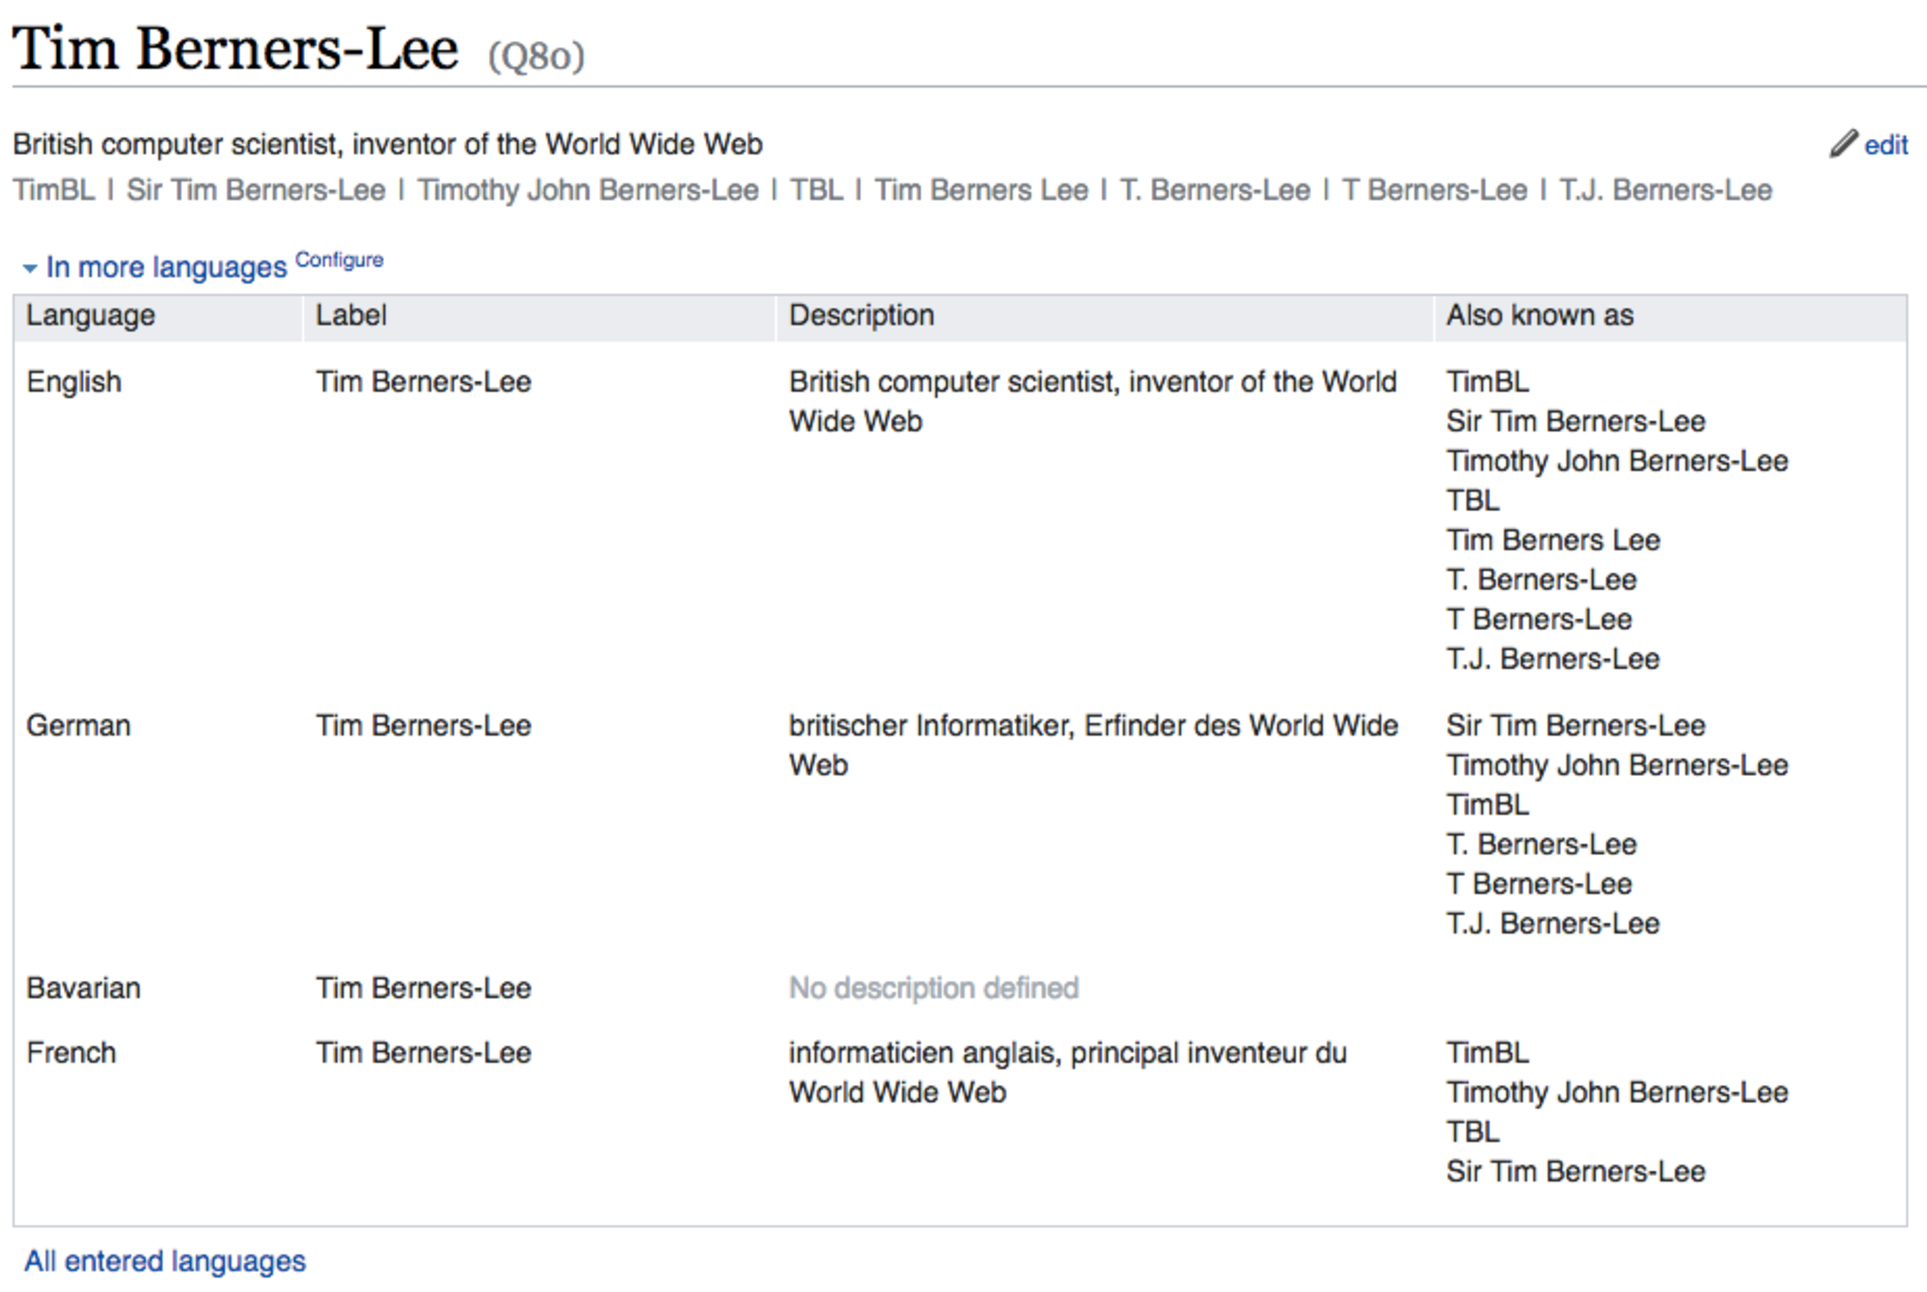
\includegraphics[width=0.75\textwidth]{graphics/wikidata_tim_berners_lee_lang}
	 \caption{Excerpt of a Wikidata page showing language properties of Tim~Berners-Lee}\label{fig:wikidata_tim_berners_lee_lang}
\end{figure}
\begin{figure}
	 \centering
	 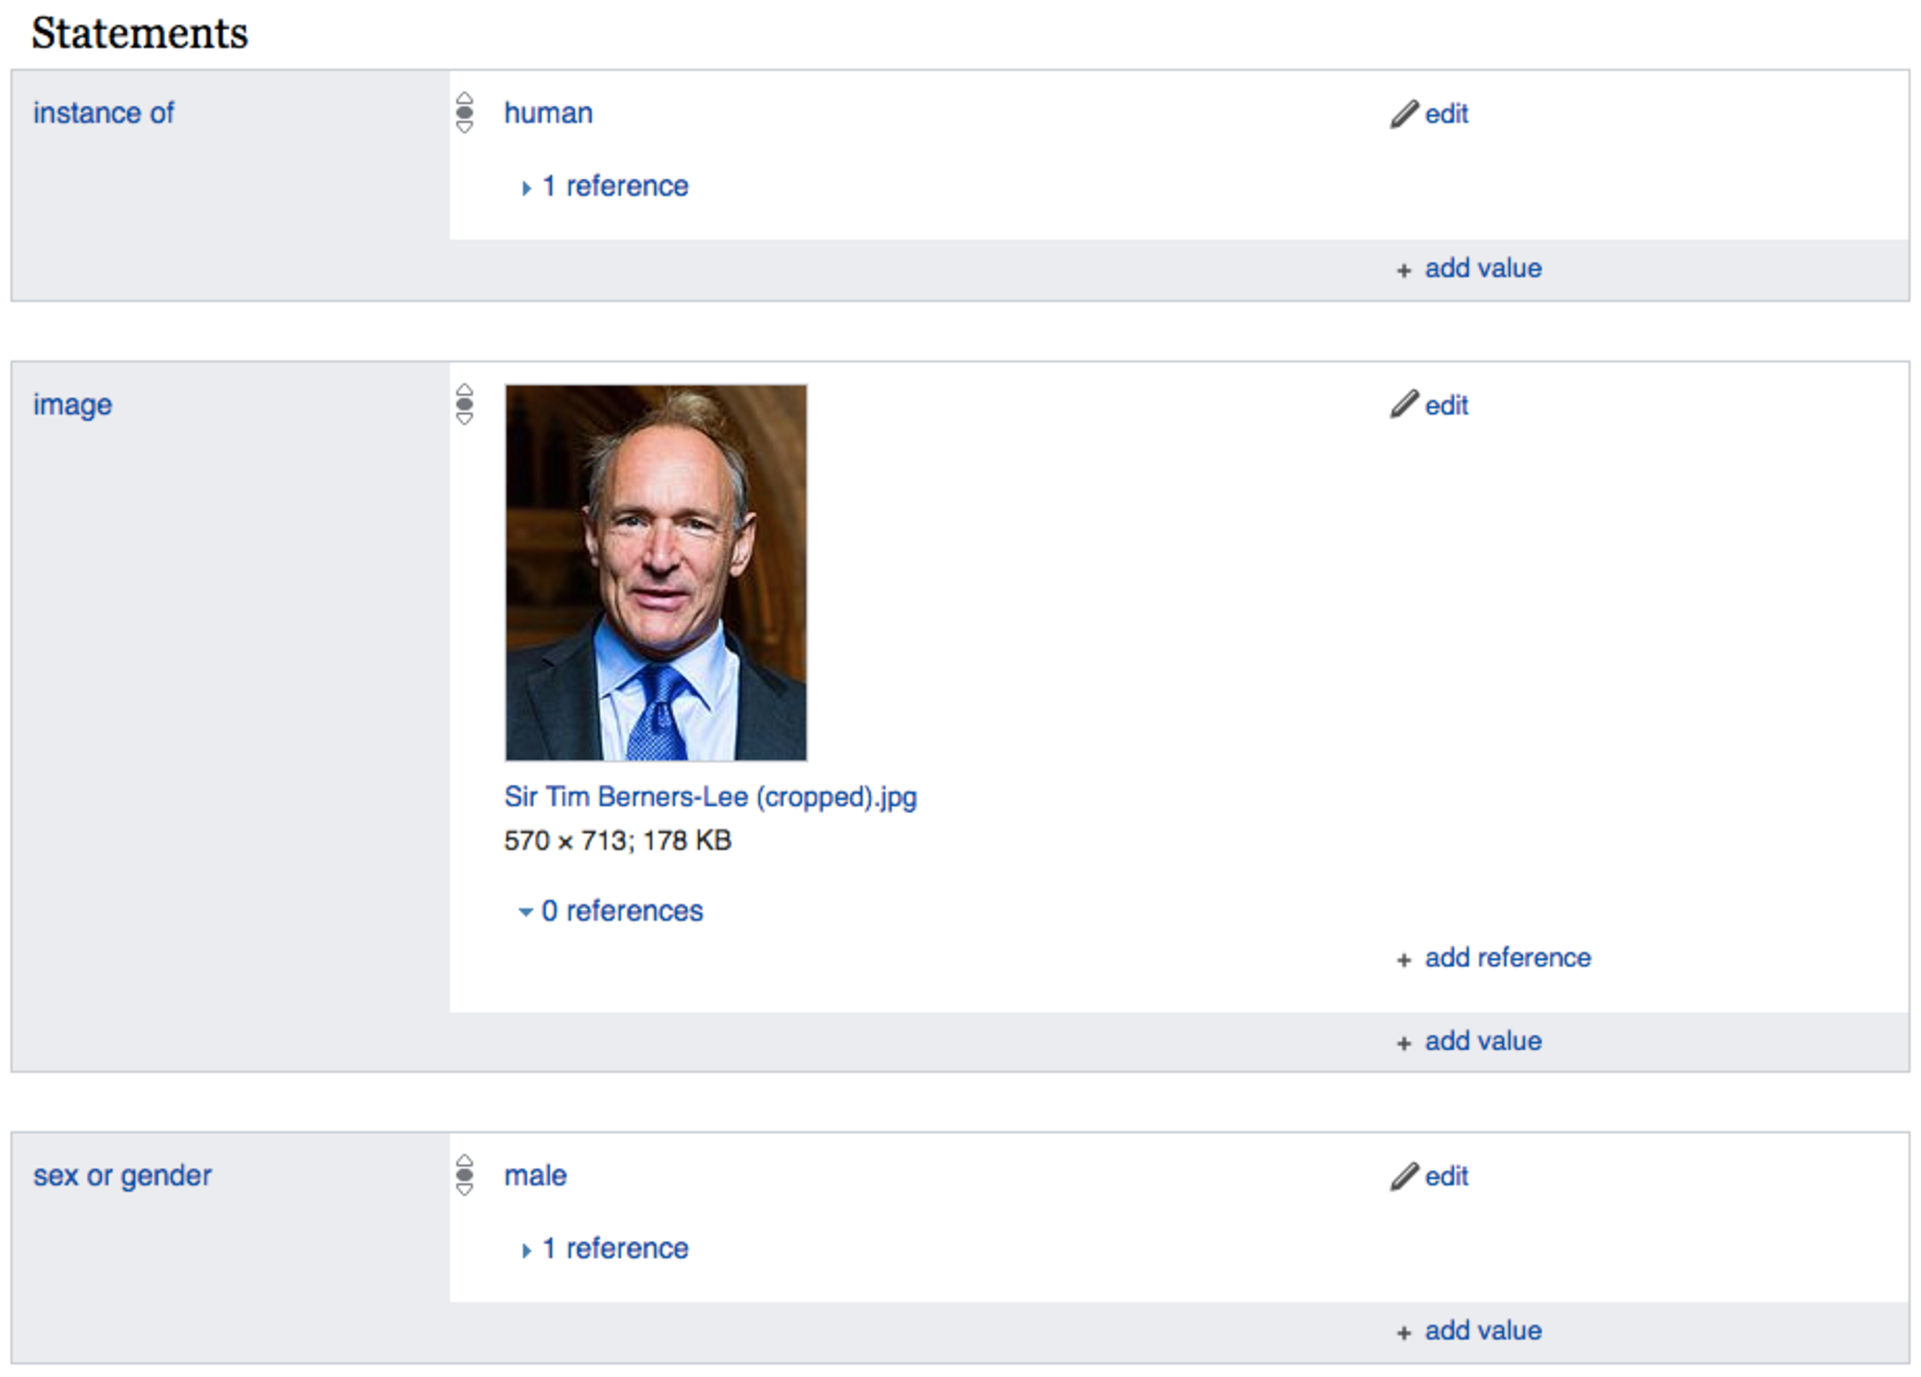
\includegraphics[width=0.75\textwidth]{graphics/wikidata_tim_berners_lee_stat}
	 \caption{Excerpt of a Wikidata page showing statements of Tim~Berners-Lee}\label{fig:wikidata_tim_berners_lee_stat}
\end{figure}
Every item~(page) has a unique identifier~(e.g. \texttt{Q80}), containing a label~(e.g. \texttt{Tim~Berners-Lee}), a brief description~(e.g. \texttt{British computer scientist, inventor of the World Wide Web}), a list of aliases~(e.g. \texttt{TimBLSir, Tim Berners-LeeTimothy, John Berners-Lee, \ldots}), a list of statements~(e.g. \texttt{instanceof, image, \ldots}) and some links. 
It is obvious that these data would perfectly fit into the Linked Data model, mapping the properties from above to RDF triples~\cite{erxleben2014}.
Wikidata content is also available in RDF encoding which is accessible at \url{http://tools.wmflabs.org/wikidata-exports/rdf/}. Unfortunately, this data is only provided via dump files\footnote{\url{https://tools.wmflabs.org/wikidata-exports/rdf/exports.html} accessed 2018/08/06} which are regularly (re-)generated. 

\paragraph{Data Storage and Indexing}
%% TODO: This needs to be done %%

\paragraph{Data Revision and Authoring} In this stage users are given the opportunity to create new or modify existing semantic information. 
Specifically, this is referred as \textit{Semantic~Content~Authoring~(SCA)} which researchers have defined as \textit{"a tool-supported
manual composition process aiming at the creation of semantic documents."}~\cite{khalili2013} More generally speaking, SCA it actually embedded in a broader ecosystem for semantic content authoring as shown in~\hyperref[fig:authoring_semantic_ecosystem]{Figure~\ref*{fig:authoring_semantic_ecosystem}}). 
\begin{figure}
	 \centering
	 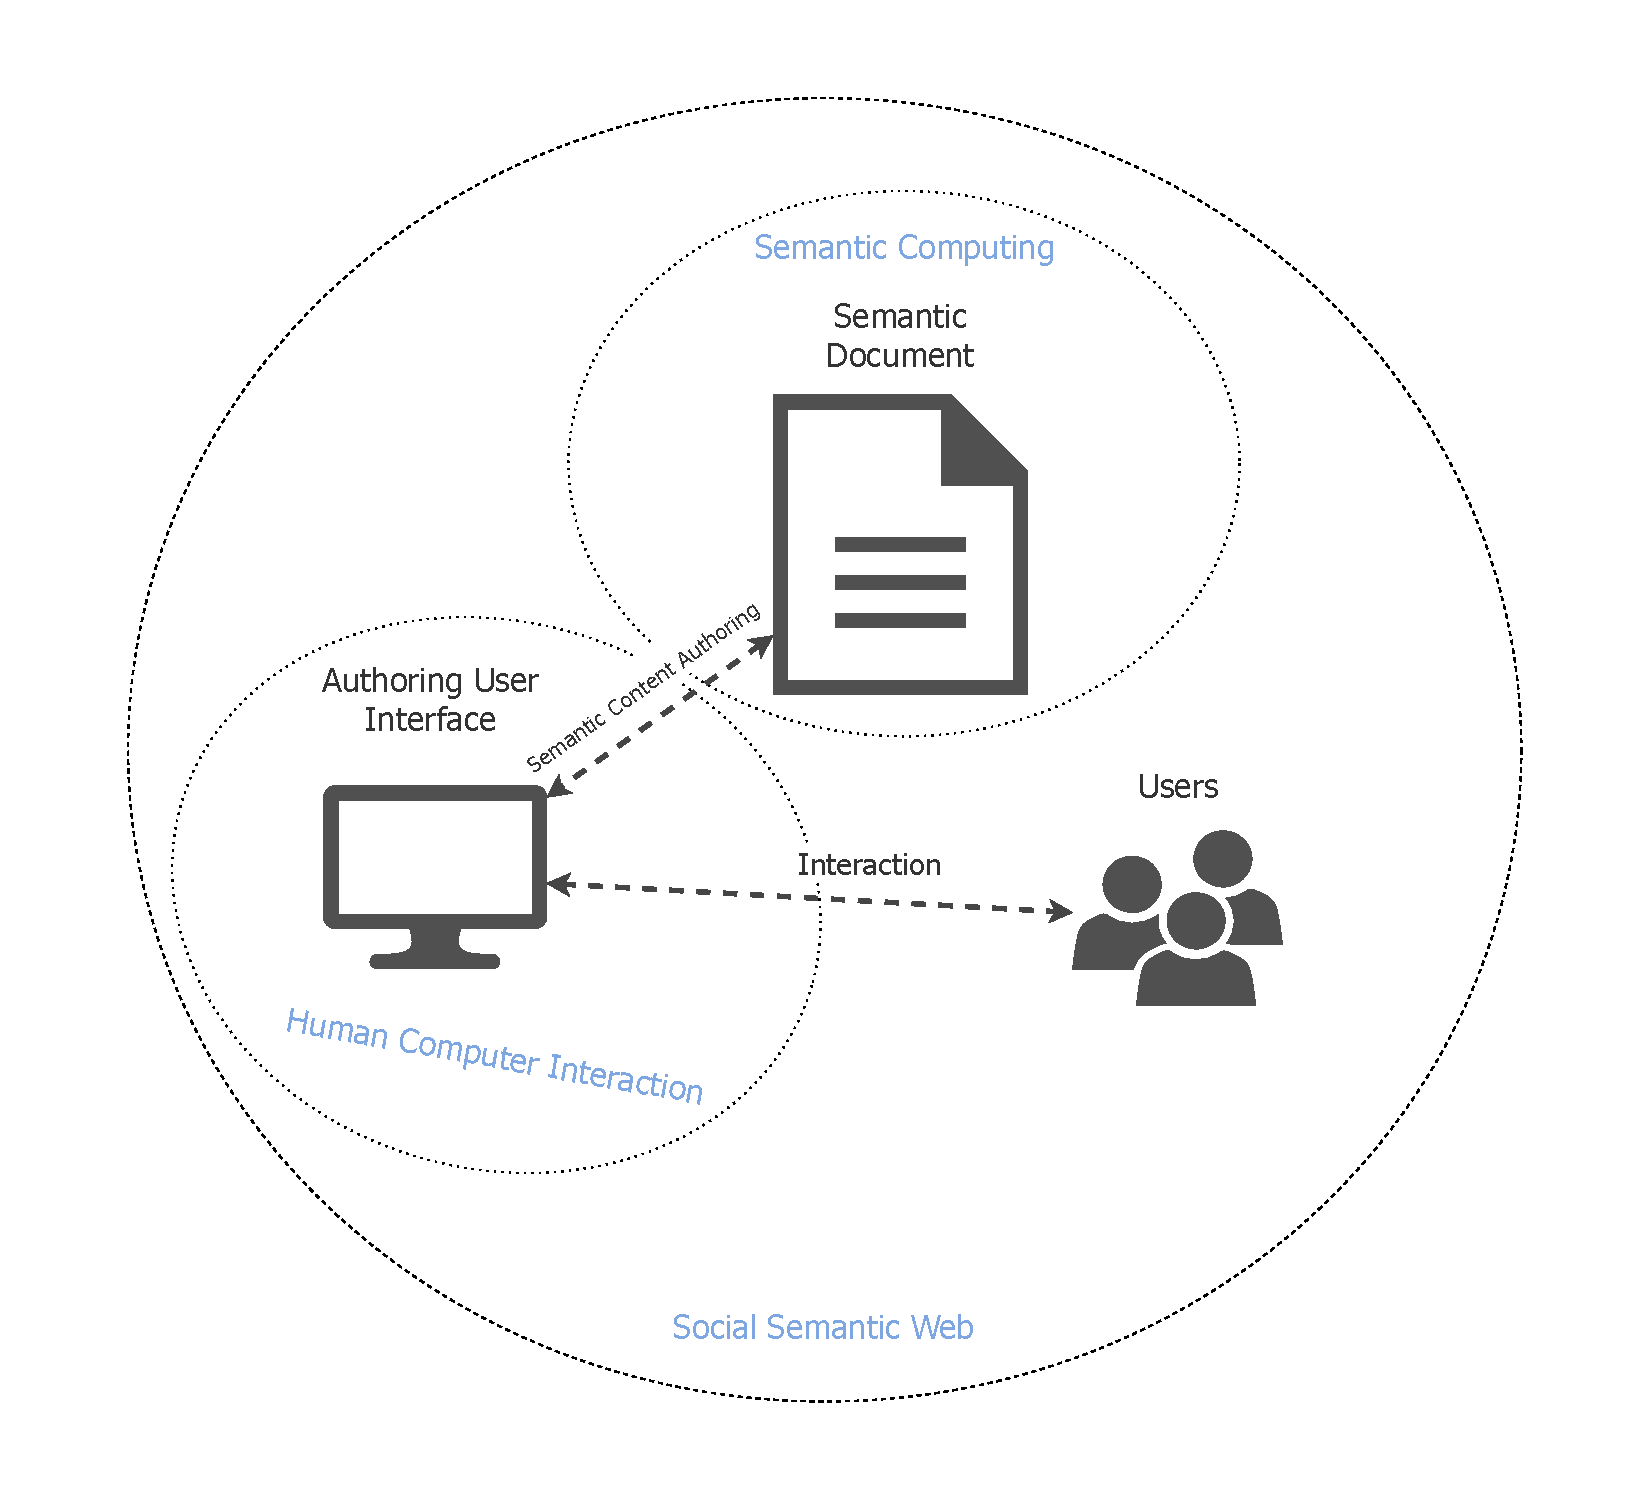
\includegraphics[width=1\textwidth]{drawio/authoring_semantic_ecosystem}
	 \caption{The ecosystem for semantic content authoring}\label{fig:authoring_semantic_ecosystem}
\end{figure}
The central entity of the semantic ecosystem is a semantic document which holds semantically enriched information. 
In information management, semantic documents serve a number of purposes such as information searching, information retrieval, information presentation, information integration, personalisation, reusability and interoperability.~\cite{khalili2013} For this reason there exists a research field dealing with major aspects of semantic content management. In particular, it covers the manipulation, creation and processing of semantic content. Users do not directly interact with semantic documents, but rather through a uniform user interface. A number of quality attributes for the assessment of UI-features of SCA-systems have been invented~\cite{khalili2013}. They are all aimed at improving the usability, a measure for the effectiveness, efficiency and satisfaction a user achieves in particular environments. 

A number of tools for authoring semantic content have been developed. A prominent example is OntoWiki~\cite{auer2006}, an open-source Semantic Wiki originally emphasising on collaboration but evolved as an ontology editor as well as a platform for knowledge acquisition. It is inspired by other Wiki systems but specifically focusing on managing knowledge bases adhering to the RDF data model. 

A different tool, incorporating Crowdsourcing capabilities in ontology development activities is Mechanical~Protege\footnote{\url{http://people.aifb.kit.edu/yt2652/mechanicalProtege/}}, which was realised as a plug-in for the ontology editor Protégé\footnote{\url{https://protege.stanford.edu/} accessed 2018/08/07}. Concretely, the following tasks are supported by the plug-in:
\begin{itemize}
	\item Creating Human Intelligence Tasks~(HIT) and submitting them to Amazon Mechanical Turk\footnote{\url{https://www.mturk.com/} accessed 2018/08/07}
	\item Monitoring the HIT's status
	\item Applying the received results to the loaded ontology
	\item Paying contributors for successful completion
\end{itemize}



%%%%%%%%%%%%%%%%%%%%%%%%%%%%
%%TODO: ADD CONTENT BELOW%%%


\paragraph{Data Linking}
TripleCheckMate: A Tool for Crowdsourcing the Quality Assessment of Linked Data, created at~\cite{acosta2013} and refined by~\cite{kontokostas2013}  (users can detect interlinking problems and others)

CrowdSPARQL - Entity resolution and Interlinking~\cite{acosta2012}

ZenCrowd: leveraging probabilistic reasoning and crowdsourcing techniques for large-scale entity linking~\cite{demartini2012}

\paragraph{Classification and Enrichment}
CrowdMap: Crowdsourcing Ontology Alignment with Microtasks~\cite{sarasua2012} (post-processing ontology alignment)

\paragraph{Data Analysis and Quality}
Urbanopoly - A Social and Location-Based Game with a Purpose to Crowdsource Your Urban Data~\cite{celino2012} (data collection \& verification \& correction)

\paragraph{Data Cleansing and Evolution}
Urbanopoly - A Social and Location-Based Game with a Purpose to Crowdsource Your Urban Data~\cite{celino2012} (data collection \& verification \& correction)

\paragraph{Data Browsing and Querying}
CrowdQ: Crowdsourced Query Understanding~\cite{demartini2013}

RDF-Hunter: Automatically Crowdsourcing the Execution of Queries Against RDF Data Sets~\cite{acosta2015}


%%%%%%%%%%%%%%%%%%%%%%%%%%%%%%
%% END CONTENT %%
